\documentclass[10pt,journal]{IEEEtran}

\usepackage{iftex}
\ifPDFTeX
  \usepackage[utf8]{inputenc}
  \usepackage[T1]{fontenc}
\fi

\usepackage{booktabs}
\usepackage{tabularx}
\usepackage{array}
\usepackage{graphicx}
\usepackage{xcolor}
\usepackage{url}
\usepackage[hidelinks]{hyperref}
\usepackage{listings}
\usepackage{caption}
\usepackage{placeins}
\usepackage{float}
\usepackage{dblfloatfix}

\captionsetup{font=footnotesize}

\lstdefinelanguage{yaml}{
  keywords={true,false,null,controls,id,description,severity,complaint_sla_hours},
  keywordstyle=\color{blue!50!black}\bfseries,
  sensitive=false,
  comment=[l]{\#},
  commentstyle=\color{gray},
  morestring=[b]',
  morestring=[b]"
}

\lstset{
  basicstyle=\ttfamily\footnotesize,
  breaklines=true,
  frame=single,
  columns=fullflexible,
  showstringspaces=false
}

\title{Making China AI Compliance Evidence Machine-Readable:\\
A Compliance-as-Code Framework for Generative AI and Deep Synthesis Services}

\author{Yuxuan Cheng%
\thanks{Technical prototype paper draft. This manuscript is not a formal publication and does not claim legal compliance certification.}}

\IEEEtitleabstractindextext{%
\begin{abstract}
AI governance increasingly depends on evidence that can be reviewed, traced, and reused across legal, operational, and engineering workflows. In China-facing AIGC and deep synthesis services, relevant obligations include model filing or disclosure, generated-content labeling, consent and scope management, content safety review, complaint handling, and personal information protection. In practice, these materials are often maintained as static documents, screenshots, spreadsheets, or disconnected operational logs. This paper presents the China AIGC Compliance Evidence Generator, a compliance-as-code research prototype that converts selected governance obligations into machine-readable controls and request-level evidence artifacts. The prototype models a synthetic AIGC actor and digital human advertising platform and evaluates each generation request against controls for consent validity, commercial-use scope, model filing metadata, visible and metadata-based labeling, content safety, and complaint handling. A seeded validation scenario assessed 1,000 synthetic generation requests, producing 800 pass, 120 review, and 80 fail outcomes; the system also generated risk records, remediation items, and 88 selected per-request evidence bundles. The prototype uses synthetic data only and does not certify legal compliance. Its contribution is a feasibility demonstration: selected China-facing AIGC governance concerns can be operationalized as machine-readable evidence pipelines rather than reconstructed after the fact through fragmented documentation.
\end{abstract}

\begin{IEEEkeywords}
AI governance, AI compliance, compliance-as-code, AIGC, deep synthesis, synthetic data, evidence engineering, privacy engineering.
\end{IEEEkeywords}
}

\begin{document}
\maketitle
\IEEEdisplaynontitleabstractindextext
\IEEEpeerreviewmaketitle

\section{Introduction}

AI governance frameworks describe what organizations should assure, but they often leave open how evidence should be generated, structured, and reviewed. The result is an implementation gap between governance requirements and operational systems. Machine-readable compliance evidence addresses this gap by representing obligations, controls, assessments, and supporting artifacts in formats that can be validated and reused by software \cite{ugarte2026machineReadableAICompliance}.

This paper adapts that logic to a China-facing AIGC service context. Chinese AI governance emphasizes generative AI service governance, deep synthesis management, AIGC labeling, algorithmic recommendation governance, model filing or registration disclosure, platform responsibility, complaint handling, and personal information protection \cite{cac2023generativeai,cac2022deepsynthesis,cac2025labeling,gb45438,pipl2021}. These obligations are not identical to high-risk conformity assessment under the EU AI Act. They are often service- and platform-centered, and they require evidence about content labeling, operational safeguards, complaint handling, and use authorization.

The technical prototype described here models an AIGC actor and digital human advertising platform. Clients submit generation requests using licensed virtual actor assets. The system evaluates whether each request has valid actor consent, whether the requested commercial use is within consent scope, whether the relevant model has filing metadata, whether the output has visible and invisible labels, whether content safety checks are appropriate, and whether complaints are handled within a synthetic service-level threshold.

The contribution is a concrete evidence pipeline rather than a legal conclusion. The prototype uses synthetic data only. It does not use real personal data, biometric data, face data, voice data, contracts, company records, or production media. Its purpose is to demonstrate the feasibility of converting selected obligations into machine-readable controls, assessment results, risk records, remediation items, and per-request evidence bundles.

\subsection{Research Questions}

To move the prototype beyond a project demonstration, the paper is organized around three research questions:

\begin{itemize}
  \item \textbf{RQ1:} Which China-facing AIGC governance obligations can be represented as machine-readable evidence controls?
  \item \textbf{RQ2:} Can a lightweight compliance-as-code prototype generate request-level evidence artifacts from synthetic platform logs?
  \item \textbf{RQ3:} What kinds of failures, risks, and remediation items can such a prototype capture in an AIGC actor and digital human service scenario?
\end{itemize}

RQ1 is addressed through the illustrative regulatory mapping and evidence profile. RQ2 and RQ3 are addressed through a seeded synthetic validation scenario and deterministic control evaluation. The study is intentionally scoped as a technical feasibility study, not as a legal validation of the selected controls.


\subsection{Related Work: From Documentation to Evidence Pipelines}

Prior work on AI documentation established important predecessors for structured transparency. Model Cards provide a template for model reporting, including intended use, performance characteristics, limitations, and ethical considerations \cite{mitchell2019modelcards}. FactSheets support supplier declarations and AI service transparency by encouraging providers to document purpose, performance, safety, security, and provenance \cite{arnold2019factsheets}. Datasheets for Datasets improve dataset documentation by recording motivation, composition, collection, preprocessing, distribution, maintenance, and provenance \cite{gebru2021datasheets}.

These formats are useful for transparency and review, but they are mostly static artifacts. They do not by themselves create continuous, request-level operational evidence tied to individual service events, labeling checks, consent status, complaint handling, and remediation workflows. A model card can describe a model, and a datasheet can describe a dataset, but an AIGC service may also need evidence that a specific generation request used an authorized actor asset, passed content checks, produced labeled output, and triggered an appropriate complaint or remediation path.

Risk-management and management-system frameworks provide another foundation. The NIST AI Risk Management Framework gives organizations vocabulary and functions for governing, mapping, measuring, and managing AI risk \cite{nist2023airmf}. AI governance maturity models build on this idea by evaluating how well organizations operationalize risk-management practices \cite{dotan2024evolving}. ISO/IEC 42001 provides an AI management system structure for organizational governance \cite{iso42001}. These frameworks are valuable for governance design, but neither provides a concrete request-level evidence pipeline for a China-facing AIGC service.

OSCAL is relevant because it shows how controls, assessment plans, assessment results, and remediation artifacts can become machine-readable in cybersecurity compliance \cite{nistOSCAL}. The source paper on machine-readable AI compliance evidence extends this logic to EU AI Act high-risk systems, arguing that compliance evidence should be represented as structured artifacts rather than reconstructed from prose after the fact \cite{ugarte2026machineReadableAICompliance}.

Content provenance and watermarking research provides a complementary line of work for AIGC labeling. C2PA defines a provenance-oriented technical standard for content credentials, while recent watermarking work explores robust signals for AI-generated media provenance \cite{c2pa2024spec,xu2024invismark}. These approaches are important for detecting or proving content origin, but they do not by themselves specify how service-level obligations such as consent scope, complaint handling, or remediation should be linked to request-level evidence bundles. Recent audit-ready engineering work similarly argues that audit artifacts can be generated as a by-product of structured development workflows \cite{koch2026agilev}; this paper applies a related evidence-by-design idea to AIGC service governance rather than to AI-assisted engineering delivery.

This paper follows that direction but adapts the evidence-pipeline logic to a different regulatory and operational setting: China-facing AIGC actor and digital human services. In this setting, selected obligations may require evidence for model filing or disclosure, visible and metadata-based labeling, consent scope, content safety, complaints, and remediation. The prototype therefore focuses on request-level evidence artifacts rather than general-purpose AI documentation alone.

\section{Regulatory Background: Chinese AI Governance as Evidence Obligations}

Chinese AI governance can be interpreted as a set of evidence obligations for providers. The Interim Measures for the Management of Generative Artificial Intelligence Services establish governance expectations for providers of generative AI services \cite{cac2023generativeai}. The Provisions on the Administration of Deep Synthesis Internet Information Services address management of deep synthesis services and synthetic media \cite{cac2022deepsynthesis}. The Measures for the Labeling of Artificial Intelligence-Generated Synthetic Content and GB 45438-2025 define expectations for visible and metadata-based identification of AI-generated synthetic content \cite{cac2025labeling,gb45438}.

The labeling regime is especially relevant for machine-readable evidence. Industry commentary distinguishes between visible labeling and implicit or metadata-based labeling \cite{pwc2025aigclabeling}. Visible labeling is user-facing and may appear as text, watermark, audio prompt, or interface notice. Implicit labeling is embedded in file metadata or comparable technical markers and is intended to support traceability and anti-tampering. The PwC report describes metadata elements such as generated-content label information, service-provider identifier, content identifier, dissemination-service provider identifier, and dissemination identifier. This supports the prototype's use of \texttt{visible\_label\_present}, \texttt{invisible\_label\_present}, and \texttt{metadata\_label\_present} as evidence fields rather than treating labeling as a single free-text disclosure.

Labeling obligations are also not limited to the point of generation. Industry commentary describes a responsibility chain across service providers, dissemination platforms, application distribution platforms, and users \cite{pwc2025aigclabeling}. Dissemination platforms may need to verify metadata, process user declarations, identify synthetic traces, and provide declaration functions. This is why the prototype frames labeling as an operational evidence obligation connected to request records, output records, and labeling checks.

Other sources provide broader context. Algorithmic recommendation provisions address platform algorithm governance \cite{cac2022algorithmic}. The Personal Information Protection Law, Data Security Law, and Cybersecurity Law define baseline expectations for personal information, data security, and network security governance \cite{pipl2021,dsl2021,csl2017}. For this prototype, these sources motivate a limited control set covering consent, scope, filing metadata, labeling, safety, and complaint handling.

\begin{table}[H]
\centering
\caption{Selected Regulatory Concerns and Evidence Artifacts}
\label{tab:regulatory-mapping}
\footnotesize
\begin{tabularx}{\columnwidth}{@{}p{0.36\columnwidth} X@{}}
\toprule
Concern & Prototype evidence focus \\
\midrule
Generative AI service governance & Assessment results and content safety checks \\
Deep synthesis governance & Generation request and output records \\
AIGC labeling & Visible, invisible, and metadata label checks \\
Consent and complaint handling & Consent scope controls, complaint records, remediation items \\
\bottomrule
\end{tabularx}
\end{table}

\FloatBarrier

\section{China AIGC Compliance Evidence Profile}

The prototype defines a compact evidence profile for machine-readable controls. Each control has a stable identifier, lifecycle phase, target type, evidence type, evaluation method, enforcement mode, threshold, responsible role, and remediation action. This profile is not a legal ontology. It is an engineering interface for connecting policy interpretation to operational logs and generated artifacts.

\begin{table}[H]
\centering
\caption{Machine-Readable Evidence Profile}
\label{tab:evidence-profile}
\scriptsize
\begin{tabularx}{\columnwidth}{@{}p{0.34\columnwidth} X p{0.26\columnwidth}@{}}
\toprule
Property & Purpose & Example \\
\midrule
\texttt{control\_id} & Stable control key & \texttt{LABEL\_CHECK} \\
\texttt{regulation\_source} & Source motivating the control & Labeling measures \\
\texttt{lifecycle\_phase} & Service phase & Publication \\
\texttt{target\_type} & Artifact evaluated & Output \\
\texttt{evidence\_type} & Expected record & Labeling check \\
\texttt{evaluation\_method} & Check logic & Metadata present \\
\texttt{enforcement\_mode} & Operational response & Review/block \\
\texttt{risk\_level} & Risk severity & Medium \\
\texttt{threshold} & Measurable rule & 72-hour SLA \\
\texttt{responsible\_role} & Operational owner & Compliance ops \\
\texttt{remediation\_action} & Follow-up action & Re-run labeling \\
\bottomrule
\end{tabularx}
\end{table}

\FloatBarrier

The profile supports repeatability. For example, a consent control can be evaluated by joining a generation request to an actor consent record and checking status, dates, usage scope, and region scope. A labeling control can be evaluated by joining an output to a labeling check. A complaint control can be evaluated by comparing complaint age or resolution time to a threshold.

\section{Architecture: Policy, Evidence, and Enforcement}

The prototype uses a three-layer architecture, shown in Fig.~\ref{fig:architecture}. The layers are intentionally simple so that the relation between policy, operational evidence, and enforcement can be inspected.

\begin{figure}[H]
  \centering
  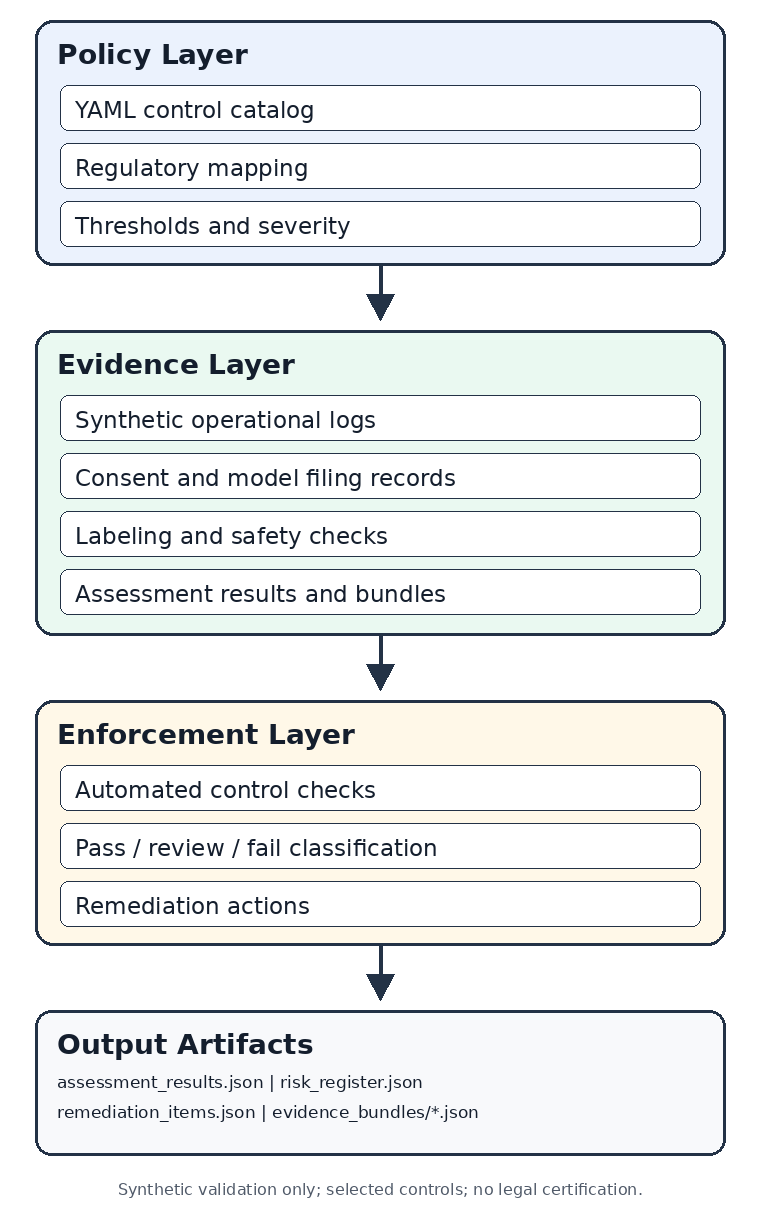
\includegraphics[width=\columnwidth]{figures/architecture_pipeline_column.png}
  \caption{Three-layer architecture for machine-readable China-facing AIGC compliance evidence.}
  \label{fig:architecture}
\end{figure}

\textbf{Policy layer.} The policy layer is a YAML control catalog. It defines control identifiers, descriptions, severity, and thresholds. In the current implementation, the policy file includes controls for consent, consent scope, model filing metadata, AIGC labeling, content safety, and complaint handling.

\textbf{Evidence layer.} The evidence layer contains synthetic operational logs and generated artifacts. Inputs include virtual actor records, actor consent records, model filing records, generation requests, output records, labeling checks, content safety checks, and complaint records. Outputs include assessment results, a risk register, remediation items, summary tables, and selected per-request evidence bundles.

\textbf{Enforcement layer.} The enforcement layer runs automated checks over the evidence layer. Each request receives a pass, review, or fail result. Review and fail conditions are aggregated into risk records and remediation items. This layer does not enforce legal compliance. It demonstrates how selected controls can be evaluated consistently and converted into reviewable evidence.
\FloatBarrier

\section{Validation Scenario: AIGC Actor and Digital Human Platform}

The validation scenario models a platform that allows clients to generate advertising videos using licensed virtual actor assets. The scenario is designed around operational evidence rather than model performance. It asks whether a particular generation request can be supported by synthetic evidence of authorization, scope, labeling, content safety, and complaint handling.

The project does not use real faces, voices, contracts, company records, or personal information. All records are synthetic. During simulated operation, the platform checks actor consent, commercial scope, revoked consent, expired consent, model filing metadata, visible AIGC labels, invisible or metadata labels, content safety status, and complaint handling status.

\subsection{Synthetic Data Generation Protocol}

The dataset was generated with a fixed seed so that the reported validation run can be reproduced from the repository. The generator creates virtual actor assets, consent records, model records, generation requests, outputs, labeling checks, content safety checks, and complaints. Failure conditions are injected deliberately to test whether the evaluator captures realistic governance exceptions rather than to estimate production incident rates. The target outcome calibration is 80 percent pass, 12 percent review, and 8 percent fail. Table~\ref{tab:synthetic-protocol} summarizes the main parameters.

\begin{table}[H]
\centering
\caption{Synthetic Data Generation Parameters}
\label{tab:synthetic-protocol}
\footnotesize
\begin{tabular}{@{}lr@{}}
\toprule
Parameter & Value \\
\midrule
Virtual actor assets & 50 \\
Consent records & 200 \\
Model records & 10 \\
Generation requests & 1,000 \\
Output records & 1,000 \\
Labeling checks & 1,000 \\
Content safety checks & 1,000 \\
Complaint records & 62 \\
Target pass rate & 80\% \\
Target review rate & 12\% \\
Target fail rate & 8\% \\
Automated tests & 14 \\
\bottomrule
\end{tabular}
\end{table}


The injected failure categories map directly to the control catalog: expired or revoked consent maps to consent validity controls; commercial use outside scope maps to consent-scope controls; missing filing metadata maps to the model-filing control; missing metadata labels map to AIGC labeling controls; unsafe content maps to content-safety controls; and overdue complaints map to complaint-handling controls. This design supports RQ2 and RQ3 by testing whether the prototype can transform synthetic operational records into assessment results, risk records, remediation items, and evidence bundles.

\section{Results}

The seeded validation run used 1,000 synthetic generation requests. The dataset contained 50 synthetic virtual actor assets, 200 synthetic consent records, 10 synthetic model records, 1,000 output records, 1,000 labeling checks, 1,000 content safety checks, and 62 synthetic complaint records. The request-level assessment produced 800 pass outcomes, 120 review outcomes, and 80 fail outcomes. The artifact builder generated 88 selected per-request evidence bundles covering pass, review, fail, and complaint-related examples. The automated test suite contained 14 tests, all of which passed in the latest recorded run.

The distribution was calibrated for a synthetic validation scenario, not for a production benchmark. The pass rate was 80.0 percent, the review rate was 12.0 percent, and the fail rate was 8.0 percent. Failure conditions included expired consent, commercial use outside consent scope, revoked consent, missing model filing metadata, missing invisible labels, high-risk content that was allowed without blocking or manual review, and overdue complaint handling.

The results support the three research questions at different levels of maturity. For RQ1, the control catalog shows that selected China-facing AIGC obligations can be expressed as inspectable control fields, although legal completeness remains outside the scope of this study. For RQ2, the prototype generates machine-readable assessment results, risk records, remediation items, and selected per-request evidence bundles from synthetic logs. For RQ3, the exception table shows that the evaluator captures several failure categories and links them to evidence sources and remediation actions.

\begin{table}[H]
\centering
\caption{Seeded Validation Summary}
\label{tab:validation-summary}
\footnotesize
\begin{tabular}{@{}lr@{}}
\toprule
Metric & Value \\
\midrule
Generation requests assessed & 1,000 \\
Pass outcomes & 800 (80.0\%) \\
Review outcomes & 120 (12.0\%) \\
Fail outcomes & 80 (8.0\%) \\
Selected evidence bundles & 88 \\
Automated tests passed & 14 \\
\bottomrule
\end{tabular}
\end{table}

\begin{table}[H]
\centering
\caption{Captured Exceptions and Remediation Artifacts}
\label{tab:exception-types}
\scriptsize
\begin{tabularx}{\columnwidth}{@{}p{0.42\columnwidth} r X@{}}
\toprule
Control category & Count & Primary artifact \\
\midrule
Consent existence / validity & 31 & risk and remediation item \\
Consent scope & 14 & risk item \\
Model filing metadata & 9 & assessment result \\
Visible AIGC label & 66 & review/fail finding \\
Invisible / metadata label & 11 & remediation item \\
Content safety & 67 & review/block finding \\
Complaint handling & 15 & remediation item \\
\bottomrule
\end{tabularx}
\end{table}

\FloatBarrier
\section{Discussion}

The prototype highlights three points. First, China-facing AI compliance evidence obligations differ from EU AI Act high-risk conformity assessment. Chinese governance sources often emphasize generative AI service management, deep synthesis, labeling, model filing or registration disclosure, platform responsibility, complaint handling, and personal information protection.

Second, selected obligations can be decomposed into executable control logic. Consent existence becomes a status and validity check. Consent scope becomes a comparison between allowed and requested use. Labeling becomes an output-level evidence check. Complaint handling becomes a threshold-based status evaluation. These controls are modest, but they show how governance obligations can become operational evidence requirements.

Third, the value of the prototype is not that it provides a legal conclusion. It does not ensure compliance, certify a service, or replace counsel. Its value is to demonstrate how selected obligations can be transformed into a structured evidence pipeline that produces assessment results, risk records, remediation items, and per-request evidence bundles for technical review.


For external submission, the next validation step is a small expert review rather than a larger synthetic dataset alone. Reviewers with backgrounds in AI governance, privacy engineering, platform compliance, or digital-content operations could assess each control for relevance, clarity, audit usefulness, and implementation feasibility. A second artifact-usefulness review could ask whether selected evidence bundles support traceability from request to consent, model, output, labeling, safety review, complaint status, and remediation. This paper reports the technical prototype and synthetic validation; those expert-review results are not yet claimed.

\section{Limitations}

This work has several limitations. The dataset is synthetic only. The prototype provides no legal certification and has no formal regulatory endorsement. It uses no real personal data, biometric data, face data, voice data, contract data, company records, or production media. It covers selected controls only and is not full Chinese AI compliance coverage. It is not sector-specific for finance, healthcare, education, media, or other regulated domains. It does not implement actual model training, production watermarking, cryptographic signing, or production-grade evidence retention. The regulatory mapping is illustrative and would require legal review before operational use. Finally, the current validation is limited to deterministic tests and synthetic logs. A workshop or preprint version can report this feasibility study, but a stronger conference or journal submission should add expert review of the control mapping and artifact usefulness.

\section{Conclusion}

This paper presents a technical prototype for machine-readable compliance evidence in China-facing AIGC actor and digital human platforms. The prototype demonstrates feasibility for translating selected AI governance obligations into controls, assessment results, risk records, remediation items, and per-request evidence bundles. Future work could expand the control catalog, integrate evidence integrity mechanisms, support more lifecycle phases, and connect the evidence profile to formal governance workflows.

\clearpage
\appendices

\section{Example Control in YAML}

\begin{lstlisting}[language=yaml,caption={Example synthetic control rule.}]
controls:
  invisible_label:
    id: AIGC_INVISIBLE_LABEL
    description: Output has invisible AIGC provenance metadata.
    severity: medium
    lifecycle_phase: publication
    target_type: output
    evidence_type: labeling_check
    evaluation_method: metadata_label_present
    enforcement_mode: block_until_labeled
\end{lstlisting}

\section{Example Evidence Bundle Schema}

\begin{lstlisting}[caption={Simplified per-request evidence bundle schema.}]
{
  "metadata": {
    "bundle_type": "per_request_synthetic_evidence",
    "data_classification": "synthetic_operational_logs",
    "contains_real_personal_data": false
  },
  "assessment_result": {
    "request_id": "REQ-0001",
    "overall_status": "pass",
    "checks": []
  },
  "actor": {},
  "consent": {},
  "model": {},
  "generation_request": {},
  "output": {},
  "labeling_check": {},
  "content_safety_check": {},
  "complaint": null
}
\end{lstlisting}

\section{Expert Review Protocol for Future Validation}

A future expert review can assess the prototype along two dimensions. For control-mapping validation, reviewers would score each control on relevance, clarity, audit usefulness, and implementation feasibility using a five-point Likert scale. For artifact-usefulness evaluation, reviewers would inspect selected evidence bundles and answer whether the bundle supports request-to-consent traceability, model and output traceability, labeling verification, safety-review traceability, complaint-status review, and remediation planning. These questions are intended as an evaluation protocol and were not used to claim expert-review results in this draft.


\FloatBarrier
\bibliographystyle{IEEEtran}
\bibliography{references}

\end{document}
